\chapter{Electrodynamique}

\section{Un exercice pédagogique}
\subsection{Générateur et circuit électrique}
%\subsection{Effet joule}
\begin{minipage}[c]{.5\linewidth}
\hspace{0.7cm}Un générateur électrique G (pile électrochimique) maintient une tension électrique (ou force électromotrice) U entre ses bornes. Cette tension produit un courant électrique I dans le circuit électrique contenant des fils de résistance négligeable et le conducteur ohmique R.
\end{minipage}
\hfill
\begin{minipage}[c]{.5\linewidth}
\begin{center}
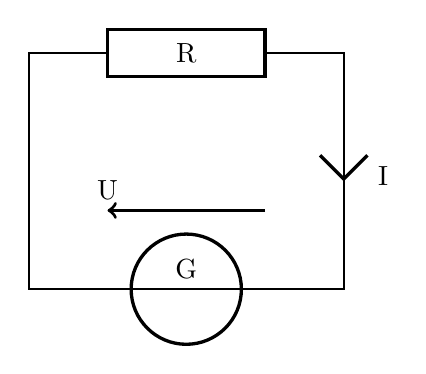
\begin{tikzpicture}
\draw [very thick] (0,0) node [above]{G} circle(0.7);
\draw [->, very thick] (1,1) -- (-1,1) node [above]{U};
\draw [thick] (-1,3) -- (-2,3) -- (-2,0) -- (2,0) -- (2,3) -- (1,3);
\draw [very thick] (-1,3.3) -- (-1,2.7) -- (1,2.7) -- (1,3.3) -- cycle;
\draw (0,3) node {R};
\draw [very thick] (2.3,1.7) node [below right]{I} -- (2,1.4) -- (1.7,1.7);
\end{tikzpicture}
\end{center}
\end{minipage}\vspace{0.5cm}

L'expérience montre que la température du conducteur ohmique s'élève, c'est l'effet Joule. Nous nous interressons aux transferts d'énergie responsable de cet échauffement :

Dans le générateur, de l'énergie électrochimique est convertie en énergie électrique, dans le conducteur ohmique de l'énergie électrique est convertie en énergie thermique. Nous souhaitons interpréter et évaluer cette dernière conversion.

Le conducteur ohmique R est cylindrique (longueur {\it l}, section {\it s}). La tension U est maintenue entre ses extrémités, il est parcouru par le courant I (le courant I est proportionnel à la tension U. C'est la loi d'Ohm : U $=$ R.I).

\begin{center}
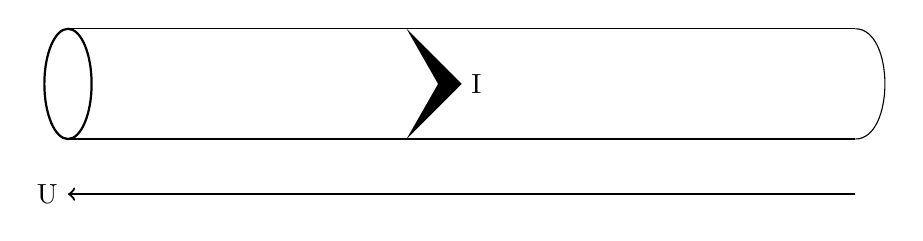
\begin{tikzpicture}
\draw[thick] (0,0) ellipse (0.3cm and 0.7cm);
\draw (0,0.7) -- (10,0.7);
\draw (0,-0.7) -- (10,-0.7);
\draw [thick,->] (10,-1.4) -- (0,-1.4) node [left] {U};
\fill (5,0) -- (4.3,0.7) -- (4.7,0) -- (4.3,-0.7) -- cycle node [right] {I};
\draw (10,0.7) .. controls (10.5,0.7) and (10.5,-0.7) .. (10,-0.7);
\end{tikzpicture}
\end{center}

La tension U est une différence de potentiel entre les extrémité du conducteur ohmique, relié par définition au champ électrique {\bf E}

\subsection{Électrons libres et champ électrique}
Au niveau microscopique, le conducteur ohmique est constitué par un réseau d'ions positifs fixes

\begin{tikzpicture}
\draw (0,0) node [color=red] {$+$};\draw (0,0) [thick, color=gray!40] circle (0.3);
\end{tikzpicture}
et d'électrons mobile
\begin{tikzpicture}
\draw (0,0) node [color=blue] {$e^-$};
\end{tikzpicture}. L'ensemble étant électriquement neutre.
\begin{center}
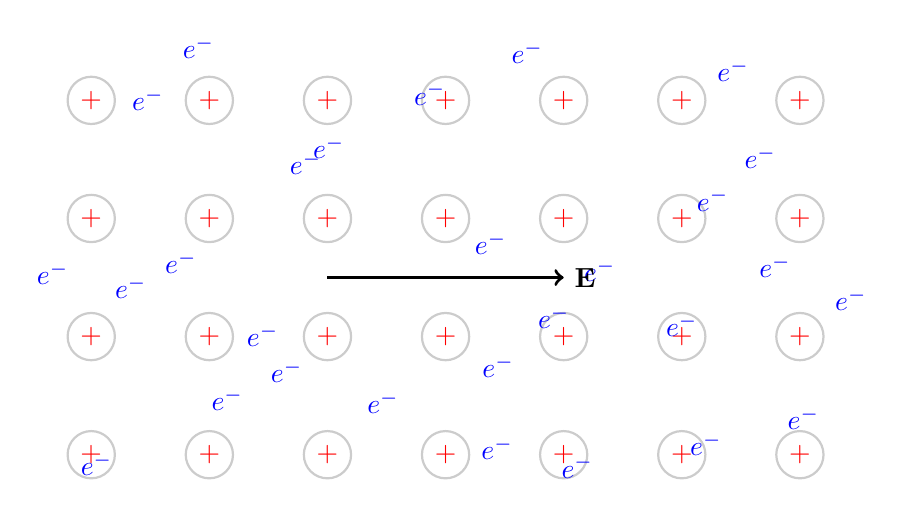
\begin{tikzpicture}
\foreach \x in {-2,-0.5,...,3}
{\foreach \y in {1,2.5,...,11}
{\draw (\y,\x) node [color=red] {$+$};\draw (\y,\x) [thick, color=gray!40] circle (0.3);
%\draw (\y+0.75+0.3*rand,\x+0.75+0.3*rand) node {$e^-$};}}
\draw (\y+0.75*rand,\x+0.75*rand) node [color=blue] {$e^-$};}}
\draw [->, very thick] (4,0.25) -- (7,0.25) node [right] {{\bf E}};
\end{tikzpicture}
\end{center}
Le courant électrique est due au mouvement d'ensemble des électrons mobiles (libres) sous l'effet du champ électrique {\bf E} ( relié par définition à la tension U
% : {\bf E} $=-\frac{\partial}{\partial\mt{x}}$V(x)$\hat{\mt{x}}$
).

Soumis à une force de la part du champ électrique, les électrons libres sont mis en mouvement. Ils subissent alors des collisions avec les ions immobile, leurs cédant une partie de leur énergie cinétique. Les ions du réseau acquièrent alors de l'énergie de vibration, se traduisant par un échauffement du conducteur.

\subsection{Champ magnétique et vecteur de Poynting}

Le courant I produit un champ magnétique : Les lignes de champs sont des cercles, centré sur l'axe du conducteur, le champ est perpendiculaire à cet axe.



